\documentclass[12pt, a4paper, fleqn, titlepage]{article}
\usepackage[utf8]{inputenc}
\usepackage{enumerate}
\usepackage{amsmath}
\usepackage{amssymb}
\usepackage{setspace}
\usepackage{array}
\usepackage{ragged2e}
\usepackage{algorithm2e}
\usepackage{graphicx}
\graphicspath{ ./ }
\usepackage[margin=1in]{geometry}

\makeatletter
\renewcommand{\@algocf@capt@plain}{above}% formerly {bottom}
\makeatother

\title{\textbf{CS 434: Parallel and Distributed Computing Lab 4}}
\author{Kweku Yamoah: 71712022}
\date{\today}

\begin{document}

\maketitle
\section*{Introduction}
    This report was generated as a requirement of Lab 4 for Parallel and Distributing computing. The report contains two sections; Part 1 and Part 2. Part 1 is the Lab where I experiment with the MaoReduce framework and my understanding in class. Part 2 is the project which focuses on implementing matrix multiplication using MapReduce algorithms. 
\section*{Part 1}
    \subsection*{MapReduce Framework \& Why}
    My selected MapReduce framework was MrJob. I chose MrJob because of the following reasons:
        \begin{itemize}
            \item it provides an easy route for writing python programs that run on Apache Hadoop.
            \item it provides an easy switch for input and output formats with a single line of code.
            \item All codes are written in a single python class which enforces the understanding of OPP concepts.
            \item it has an extensive documentation with examples as reference, which, makes learning of the framework easy.
        \end{itemize}
    Installing MrJob was easy because it require running a command with the python pip package. However, understanding the documentation and how to submit my first job took some time to understand.

    \subsection*{Word-count Algorithm}
        Firstly, the word-count algorithm prints out the frequency of each word in a text file.

        The word count algorithm inherited the \textbf{MrJob} class to implement a job that executes the task. This job class required the implementation of the methods \textbf{mapper\_init, configure\_args, mapper and reducer}. 
            \begin{itemize}
                \item The \emph{configure\_args} method creates command-line options. I used tis to pass the stop words file as a command line argument.
                \item The \emph{mapper\_init} method initializes or setups the resources that the mapper method needs. I read the stop words and converted the words to a python set in this method.
                \item \emph{mapper} method splits every sentence from the text file into words.
                All the stop words are removed before further processing. The method
                finally returns a key-value pair consisting of the word as the key and a one as the value for every word. E.g., word, 1.
                \item \emph{reducer} method in this program acts as a combiner and a reducer
                at the same time. This method finds the occurrences of each word in the
                text by summing up the results from the mapper method passed to it.
                The output of the reducer method is a key-value pair containing a word
                as the key and the value as the number of times it appears in the text.
            \end{itemize}
    \subsection*{Running the Program}
            The program needs some requirements to be satisfied first before running.
                \begin{itemize}
                    \item The program requires python 3 or later to run.
                    \item The program requires the correct command-line arguments to be passed before it can run.
                    \item The program must be run on a Linux subsystem; Ubuntu is preferred.
                \end{itemize}
            
            To run the program type this in your terminal whilst ensuring that you are in the directory which contains the program files;
            \textbf{python3 mrjob\_wordcount.py $<$input.txt - -stop-words$=$stop\_words.txt}

\section*{Part 2}
In this section I implement matrix multiplication using the MapReduce framework MrJob with block-block partitioning. I assume that my matrices are of dimensions $N * N$ and $P $ which is the number of processors is an even square number.
\subsection*{Overview of Algorithm}
    The first step of the algorithm is to partition the matrices into blocks. Matrix A is split into $\sqrt{P}$ blocks along the rows and matrix B is also split into $\sqrt{P}$ blocks along the columns. After, $P = \sqrt{P} * \sqrt{P}$ tasks are spawned for the mapping and reduce phases.
\subsubsection*{Pseudocode of Map and Reduce Phases}
    \begin{algorithm}[H]
        \CommentSty{Brief: Maps a given N x N matrix with block partitioning}\\
        \CommentSty{Input: matrix file, size(where size = N)}\\
        \CommentSty{Output: key value pairs for row block and column block}\linebreak

        %Main Algorithm
        \For{i in generate\_partitions.rowMajor(matrix,bands,offset)}{
            \For{j in generate\_partitions.columnMajor(matrix,bands,offset)}{
                yield str(count), i
                yield str(count), j
            }
        }

        \begin{center}
            \caption{mapper\_raw(self,input\_file,input\_uri)}
        \end{center}
    \end{algorithm} 

    \begin{algorithm}[H]
        \CommentSty{Brief: Reduces a given N x N matrix with block partitioning}\\
        \CommentSty{Input: key value pairs)}\\
        \CommentSty{Output: matrix multiplication for row block and column block}\linebreak

        %Main Algorithm
        \For{i in values}{
            put i in localList
        }

        \ForEach{row in localList}{
            \ForEach{column in localList}{
                answer.append(row * column)
            }
        }
        yield key, answer
        \begin{center}
            \caption{reducer(self,key,values}
        \end{center}
    \end{algorithm} 

\subsection*{Performance Results}
    The table below shows the performance of the two versions as implemented in the python programming language. The largest matrix that was computed was a 2,048 element matrix. No larger matrices were attempted due to hardware limitations.
        \begin{center}  
            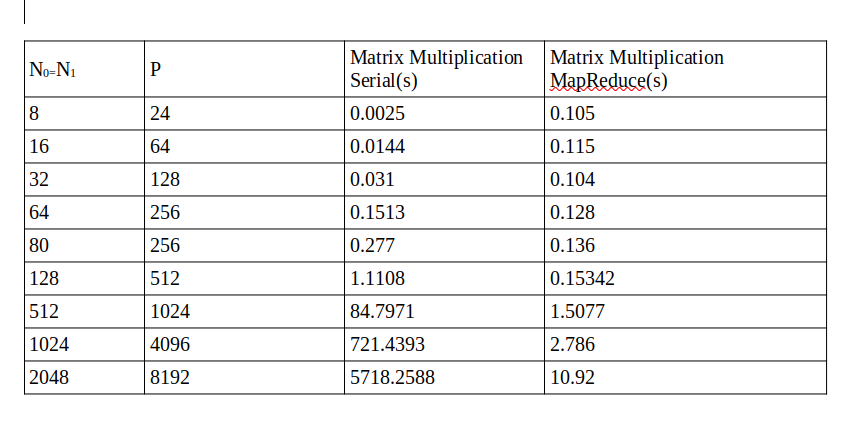
\includegraphics[width= 18cm,height = 10cm, keepaspectratio,scale=0.5]{performance-mapreduce}
        \end{center}

    After generating the comparative table, I observed that for small sizes of N the serial Implementation of the matrix multiplication algorithm executed faster. However, as N grew exponentially, the parallel implementation in MapReduce executed faster than the serial implementation. This goes to show the importance of parallel computing and message passing communications in Computing.

    Here is a graph visualising the difference between the serial implementation and the MapReduce implementation as the matrix size increases.
        \begin{center}  
            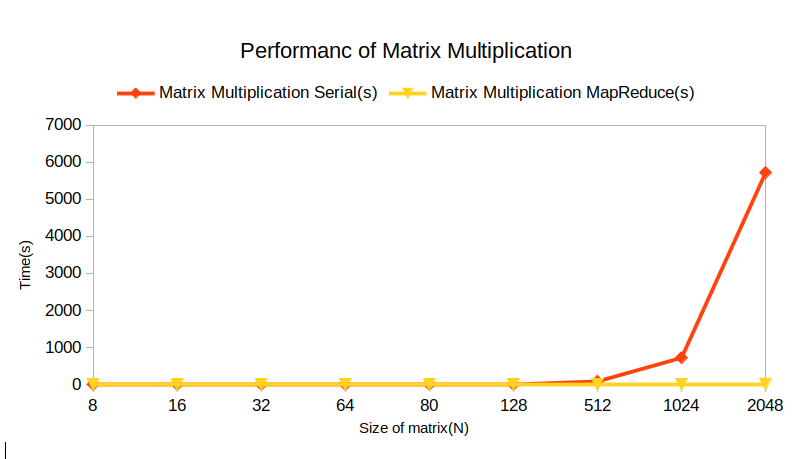
\includegraphics[width= 18cm,height = 10cm, keepaspectratio,scale=0.5]{graph}
        \end{center}

\subsection*{Running the Program}
    The program needs some requirements to be satisfied first before running.
    \begin{itemize}
        \item The program requires python 3 or later to run.
        \item The program requires the correct command-line arguments to be passed before it can run.
        \item The program must be run on a Linux subsystem; Ubuntu is preferred.
    \end{itemize}
    First one needs to run the serial version of the code before the parallel version. To run the serial version run the command; \textbf{python3 matrix\_mults.py N}; where \emph{N(matrix size)=} 16,64,80,128 etc.

    To run the program type this in your terminal whilst ensuring that you are in the directory which contains the program files;
    \textbf{python3 mrjob\_matrixmult.py matrix.txt - -P=n}; where \emph{n(number of processors)=} 64,256,512 etc
\end{document}